\documentclass[../../DD.tex]{subfiles}
\begin{document}
\section{Introductory Pages \label{sect:2.1}}
	\subsection{Musical Instruments}
		Musical Instruments introductory page contains a list of traditional musical instruments that are interesting from the association's point of view. Each instrument is represented by its name and a picture, both of them are links to the instrument page. Two filters allow to show to the user a subset of these instruments: the first one filters them by type (e.g. Flutes, Aerophone...), the second one selects them by the region they come from.
		\newline
		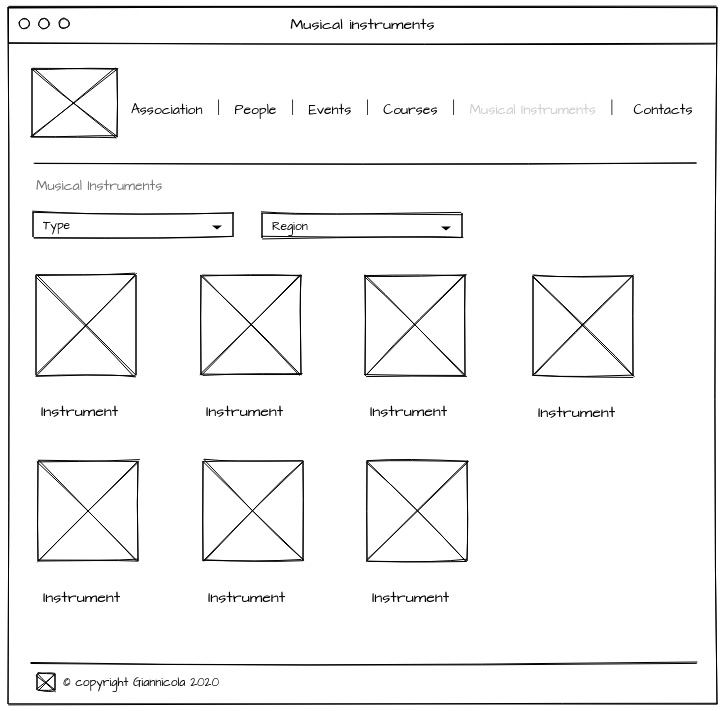
\includegraphics[width=\textwidth,height=\textheight,keepaspectratio]{Wireframes/IntrMusicalInstruments.jpg}

	\subsection{Courses}
		This introductory page contains a list of the courses hold by [name] association. Each course has an image and a title that bring to the single course page, to read more information about it.
		\newline
		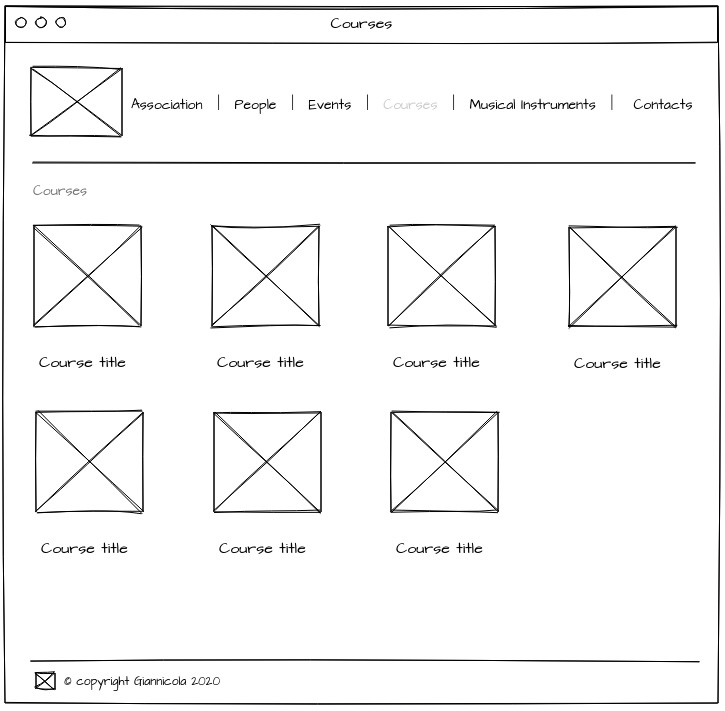
\includegraphics[width=\textwidth,height=\textheight,keepaspectratio]{Wireframes/IntrCourses.jpg}

	\subsection{Events}
		Events page is divided into two main subsections containing next and past events. In this page, all events are represented by an image, a title and a short description that gives the idea of what the event is about. From this page it is possible to open the single-event pages to have more details about it. Through a filter, the user can select the events of a specific month, to have an immediate view of what the association is organizing in a defined time section.
		\newline
		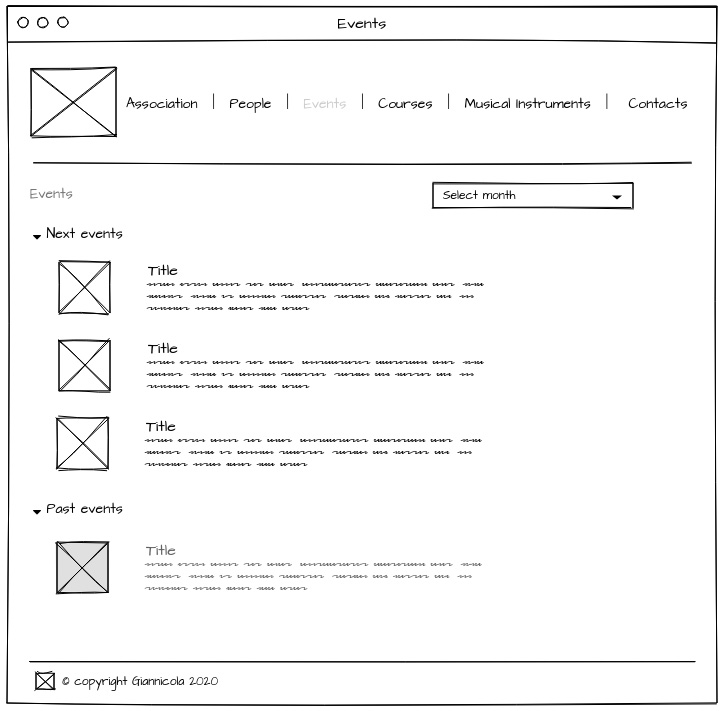
\includegraphics[width=\textwidth,height=\textheight,keepaspectratio]{Wireframes/IntrEvents.jpg}
	\end{document}
